\section{Technische Grundlagen}
\subsection{Robotik} % Manuel ca. 8

\subsubsection{Grundlagen}
\subsubsection{Mobile Roboter}
\subsubsection{Antriebsarten}
\subsubsection{Sensorik}
\subsubsection{LEGO Mindstorm}

\newpage
\subsection{App Entwicklung} %Simon ca. 8

\begin{wrapfigure}{r}{0.45\textwidth}
	\begin{center}
		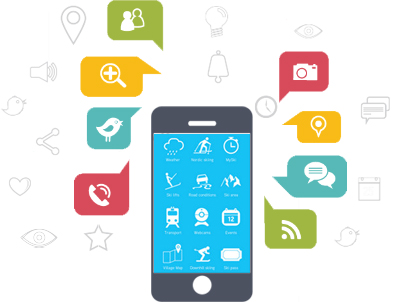
\includegraphics[width=0.4\textwidth]{images/technische_grundlagen/App-Development.jpg}
	\end{center}
	\caption{App Entwicklung}
	\label{fig:appentwicklung}
\end{wrapfigure}

Eine \gls{app} ist ein ausführbares Programm für mobile Geräte, wie Smartphones oder Tablets. Um eine App für ein mobiles Gerät zu entwickeln, müssen wie für andere Anwendungen im Voraus Anforderungen definiert werden, nach denen sich die entsprechende Softwareentwicklung richtet. Je nach festgelegten Anforderungen, können verschiedene Möglichkeiten genutzt werden. Allgemein kennt die App Entwicklung drei verschiedene Arten, die native, web und hybride Entwicklung.\\
In der nativen Entwicklung werden die direkten Ressourcen des Gerätes verwendet. Dazu gehört die Laufzeitumgebung, Bibliotheken, Geräteschnittstellen und andere APIs. Der Vorteil hierbei ist, dass diese Entwicklungen für Betriebssystem optimiert sind, da sie auf die vorhandenen Schnittstellen aufbauen können und daher komplexere und rechenintensivere Anwendungen ermöglichen.(Zitat ) die 


Ein Beispiel ist hierfür eine native Android Entwicklung durch Java und Googles Android Studio, wobei die direkten Ressourcen von Android genutzt und somit auch die vorhandenen UI Elemente und Schnittstellen zur Verwendung kommen, die Android Nutzer gewohnt sind.\\
Die web Entwicklung arbeitet hingegen zur nativen Entwicklung mit systemübergreifenden Ressourcen und greift dabei auf gängige Webtechnologien, wie HTML, CSS und Javascript zurück. Die App wird hierbei nicht wie normale Anwendungen direkt auf dem System des Gerätes ausgeführt, sondern kommt in dessen Browser zur Ausführung.

\subsubsection{Arten}

\subsubsection*{Web Apps}
\subsubsection*{Native Apps}
\subsubsection*{Hybride Apps}

\subsubsection{Plattformübergreifende Programmierung}

\subsubsection*{Xamarin}
\subsubsection{Mono}
\subsubsection{.Net Framework}

\subsection{Java} %Gemeinsam ca. 2

\subsubsection{Grundlagen}
\subsubsection{Java Runtime Environment}

\subsection{Kommunikation} %Manuel ca. 5

\subsubsection{Grundlagen}
\subsubsection{TCP/IP}
\subsubsection{Wifi}
\subsubsection{Datenaustausch} %(JSON und Serialisierung)

\section{Theoretische Grundlagen}

\subsection{Schwarmverhalten}
\subsubsection{Allgemein}
\subsubsection{Vorbilder aus dem Tierreich}
% Fische, Bienen, Ameisen
\subsubsection{Szenarien}
\subsubsection{Algorithmen}